%%%%%%%%%%%%%%%%%%%%%%%%%%%%%%%%%%%%%%%%%%%%%%%%%%%%%%%%%%%%%%%%%%%%%%%%%%%%%%%%
%2345678901234567890123456789012345678901234567890123456789012345678901234567890
%        1         2         3         4         5         6         7         8

\documentclass[letterpaper, 10 pt, conference]{ieeeconf}  % Comment this line out if you need a4paper
\usepackage{graphicx}
\graphicspath{{figs/}}                     
%\documentclass[a4paper, 10pt, conference]{ieeeconf}      % Use this line for a4 paper

\IEEEoverridecommandlockouts                              % This command is only needed if 
                                                          % you want to use the \thanks command

\overrideIEEEmargins                                      % Needed to meet printer requirements.

%In case you encounter the following error:
%Error 1010 The PDF file may be corrupt (unable to open PDF file) OR
%Error 1000 An error occurred while parsing a contents stream. Unable to analyze the PDF file.
%This is a known problem with pdfLaTeX conversion filter. The file cannot be opened with acrobat reader
%Please use one of the alternatives below to circumvent this error by uncommenting one or the other
%\pdfobjcompresslevel=0
%\pdfminorversion=4

% See the \addtolength command later in the file to balance the column lengths
% on the last page of the document

% The following packages can be found on http:\\www.ctan.org
%\usepackage{graphics} % for pdf, bitmapped graphics files
%\usepackage{epsfig} % for postscript graphics files
%\usepackage{mathptmx} % assumes new font selection scheme installed
%\usepackage{times} % assumes new font selection scheme installed
%\usepackage{amsmath} % assumes amsmath package installed
\usepackage{amsmath}
\usepackage{graphicx}
\usepackage{hyperref}
%\usepackage{amssymb}  % assumes amsmath package installed

\title{\LARGE \bf
Robot Localization on NCLT dataset using ORB-SLAM3 and Graph-Based Sensor Fusion
}


\author{Zikun Zhou$^{1}$, You Hu$^{1}$, Yichen Song$^{2}$, Yang-Lun Lai$^{1}$ and Apoorva Roy$^{3}$%
\thanks{$^{1}$Zikun Zhou, You Hu and Yang-Lun Lai are with the Department of Electrical and Computer Engineering, University of Michigan, Ann Arbor, MI, 48109, USA
        {\tt\small [kennyzzk|youhu|yanglunl]@umich.edu}}%
\thanks{$^{2}$Yichen Song is with the Robotics Institute, University of Michigan, 
        Ann Arbor, MI 48109, USA
        {\tt\small yichens@umich.edu}}%
\thanks{$^{3}$Apoorva Roy is with the Department of Mechanical Engineering, University of Michigan, Ann Arbor, MI 48109, USA
        {\tt\small apoorvar@umich.edu}}%
\thanks{$^{*}$Equal Contribution}
}



\begin{document}


\maketitle
\thispagestyle{empty}
\pagestyle{empty}


%%%%%%%%%%%%%%%%%%%%%%%%%%%%%%%%%%%%%%%%%%%%%%%%%%%%%%%%%%%%%%%%%%%%%%%%%%%%%%%%
\begin{abstract}

In this project, we used ORB-SLAM3 and the graph-optimization-based sensor fusion based on the incremental smoothing technique (iSAM2) in GTSAM library to perform localization on the University of Michigan North Campus Long-Term Vision and Lidar Dataset (NCLT). We first pre-processed the images in the dataset and used the sequence of images and IMU measurements as inputs for ORB-SLAM3 to generate the estimated trajectory. Subsequently, to further improve the robustness and accuracy of the localization result, graph-optimization-based sensor fusion was used, which combined the estimated trajectory of ORB-SLAM3 with the precomputed odometry. The odometry information computed from IMU and wheel encoder data was used, as it provides real-time information about the robot's acceleration and angular velocity, which can be transformed into the translation and rotation information of the robot. Our open-source code and the presentation video can be found at \href{https://github.com/kennyzzk/Robot-Localization-on-NCLT-dataset-using-ORB-SLAM-III-and-Graph-Based-Sensor-Fusion}{this repository} (licensed under GPL-3.0 License).

%The purpose of graph optimization is to minimize the distortion of image as a result of pinhole camera's nature.

\end{abstract}


%%%%%%%%%%%%%%%%%%%%%%%%%%%%%%%%%%%%%%%%%%%%%%%%%%%%%%%%%%%%%%%%%%%%%%%%%%%%%%%%
\section{INTRODUCTION}

Simultaneous Localization and Mapping (SLAM) is a technique for obtaining the map of an unknown environment and keeping track of the location simultaneously. SLAM using cameras only has become popular in recent years, and it is called visual SLAM (vSLAM) as the only input it uses is visual information. The early work of vSLAM, called the “feature-based approach,” used a monocular camera and was based on tracking and mapping feature points. “Direct approach” vSLAM algorithms deal with texture-less or feature-less surroundings by not detecting feature points instead of working with the entire image for tracking and mapping. Further, as inexpensive RGB-D sensors became widely available, vSLAM algorithms with both a monocular image and its depth were developed. vSLAM algorithms are fundamentally composed of five modules \cite{intro}: initialization, tracking, mapping, relocalization, and global map optimization. Algorithms vary in the methodologies that they employ for each module. vSLAM, visual odometry (VO), and online structure from motion work together to estimate the camera motion and 3D structure in an unknown environment. Odometry is the estimation of sequential changes in sensor positions over time using sensors such as wheel encoders to compute relative sensor movement. Based on \cite{1} and \cite{2}, vSLAM is a combination of camera-based visual odometry and global map optimization. Structure from motion (SfM) is a methodology to estimate camera motion and the 3D structure of the environment in a batch manner. vSLAM, VO, and SfM share many common properties. Feature-based methods are of two kinds – filter-based and bundle adjustment (BA) based. Monocular SLAM is a filter-based vSLAM method in which camera motion and 3D structure of an unknown environment are simultaneously estimated using an extended Kalman filter (EKF).

Low cost and high accessibility make vSLAM prevail. However, its performance is not very promising under extreme conditions such as sharp turns or illumination changes which is proven by a study of vSLAM’s performance on the University of Michigan North Campus Long-Term Vision and Lidar dataset (NCLT) \cite{3}. In this case, more information is needed to increase the performance of vSLAM. ORB-SLAM3 \cite{orbslam3} is the state-of-the-art visual-inertial SLAM algorithm, which tightly fuses the IMU information into the vSLAM system. In this project, we first pre-process the NCLT dataset to make it work on ORB-SLAM3. Then, we design a system that uses ORB-SLAM3 \cite{orbslam3} as the base structure and optimize the estimated trajectory with graph-based sensor fusion. Specifically, we loosely couple the estimated trajectory of ORB-SLAM3 with the precomputed odometry fused from the wheel encoder information and IMU information to reduce the trajectory estimation error.

% Low cost and high accessibility make Monocular Visual Simultaneous Localization and Mapping (SLAM) prevailed.  However, the performance of the algorithm is not very promising under extreme condition such as sharp turn or illumination change which is proofed by a study of VSLAM’s performance on the NCLT dataset \cite{3}. In this case, more information are needed in order to increase the performance of VLSAM's performance. In this project, we uses ORB-SLAM3 \cite{orbslam3} as the base structure and integrate it with sensor fusion. To be specific, apart from the image information, we also combine the data from IMU reading to further increase the accuracy of trajectory prediction.

\section{RELATED WORKS}


\subsection{Visual (Inertial) SLAM}
As the environment becomes large, MonoSLAM suffers from high computational costs. Work on visual odometry by Mouragon et al. \cite{Mouragon} and Klein and Murray \cite{Klein} was the first real-time application of bundle adjustment, known as Parallel Tracking and Mapping (PTAM). After PTAM was introduced, most of the vSLAM algorithms followed the frame of Tracking and Mapping (TAM). This algorithm provided simple yet effective techniques for keyframe selection, feature mapping, point triangulation, camera localization for every frame, and relocalization after tracking failure. Though PTAM is better than MonoSLAM, it is still limited to small-scale operation and suffers from disadvantages, such as lack of loop closing and adequate handling of occlusions, low invariance to viewpoints of the relocalization, and the need for human intervention for map bootstrapping. Pose graph optimization can be used to solve the issue of loop closure in BA-based methods.

When a stereo camera is used as the vision sensor in vSLAM systems, the scale of the coordinate system is fixed and known. However, in MonoSLAM, the scale remains ambiguous and varies if global BA is not carried out. In order to rectify this scale drift problem, the camera poses have to be optimized. Therefore, a complete version of feature-based monocular vSLAM called ORB-SLAM \cite{7} was developed, which includes BA, vision-based closed-loop detection, and 7DoF pose graph optimization. ORB-SLAM stands for Oriented Fast and Rotated Brief Simultaneous Localization and Mapping. It provides short- and medium-term tracking.


Monocular SLAM and Stereo SLAM suffer from a small field of view (FOV) and are interrupted by dramatic illumination changes, occlusions, moving objects, and sharp turns. Even if a panoramic camera can capture a 360° degree view, vSLAM is not robust as visual sensors are defective, overly sensitive to illumination, and unable to operate in textureless and/or dynamic scenes. Therefore, visual-inertial odometry (VIO) has become a widespread technique in SLAM due to the complementary nature of the inertial measurement unit (IMU) and visual sensor. The IMU substantially improves tracking performance \cite{8} and visual information helps eliminate the bias of the accelerometer and gyroscope. The methods of fusing the inertial and visual measurements utilize various derivatives of Kalman Filters and can be categorized into loosely coupled methods and tightly coupled methods. In loosely coupled integration, the output of the visual motion estimation stage is used as the measurement \cite{12}. Rotational and translational components of visual motion estimates are used separately or together, depending on the construction of the integration filter. The filter requires only the uncertainty of the visual motion estimate. The tightly coupled VIO methods that fuse the raw visual and inertial measurements can be extended Kalman filter (EKF)-based methods and graph-based methods that marginalize the past states and obtain a more precise pose by using bundle adjustment with the raw inertial measurements and visual measurements. However, one shortcoming of VIO is that the IMU error needs to be integrated into the optimization. Reintegration of the instant IMU measurements into each optimization iteration is time-consuming. To bypass repeated IMU propagation, Forster et al. \cite{12} proposed a method called preintegration. IMU preintegration condenses a large number of measurements into a single relative motion constraint, thereby providing observations that are independent of the visual measurement for constraining the camera pose estimation and also helping to estimate the absolute scale, roll, and pitch angles \cite{3}. 

\subsection{Related datasets}

Currently, the robotics community has released a number of public datasets on the internet. The EuRoC \cite{euroc} and TUM-VI \cite{tumvi} datasets are widely-used datasets on indoor scenes that the ORB-SLAM runs in. These datasets contain stereo images, IMU measurements, and accurate motion ground-truth, which enable ORB-SLAM to perform Visual, Visual-Inertial, and Multi-Map SLAM. The NCLT dataset \cite{NCLT} consists of omnidirectional imagery, 3D lidar, planar lidar, GPS, and proprioceptive sensors for odometry collected using a Segway robot. This dataset was repeatedly collected indoors and outdoors, and its completeness facilitates this project to extend the ORB-SLAM3 with tightly coupled and loosely coupled sensor fusion. The Málaga urban dataset \cite{11} is gathered entirely in urban scenarios with a car, while the MIT Stata Center Dataset \cite{14} contains vision (stereo and RGB-D), laser, and proprioceptive data collected by a robot within a building. These are valuable datasets for researchers working on long-term autonomy.

\section{METHODOLOGY}
\subsection{Odometry model}
In NCLT dataset \cite{3}, odometry is calculated with an extended Kalman filter which uses a differential-drive process model that integrates measurements from wheel encoders and a single-axis fiber optic gyro (FOG) that observes change in heading. And the measurement model is derived from IMU data including roll, pitch, and body-frame angular rates.

Specifically, we define the state variable as $\textbf{x}_t=[x,y,\phi,\theta,\psi,p,q,r]$, where ${[x,y]}^T$ is the robot's translation position in the local frame, ${[\phi,\theta,\psi]}^T$ are the Euler angles representing robot's orientation, and ${[p,q,r]}^T$ represents the body frame angular rates. The process model predicts the position and heading of the robot using differential drive model, where the input is defined as $u_t={[v_r,v_l,{\delta}_\psi]}^T$. Here, $v_r$ and $v_l$ represent the speeds of the left and right wheels and ${\delta}_\psi$ represents the heading change of the robot. And the mapping of Euler rates to body rates is given by following rotation sequence $rotz(\psi)\rightarrow{roty(\theta)}\rightarrow{rotx(\phi)}$:

\begin{align}
\begin{split}
\begin{bmatrix} p\\q\\r\end{bmatrix}
&=
\begin{bmatrix} \dot{\phi}\\0\\0\end{bmatrix}
+
rotx(\phi)\begin{bmatrix} 0\\\dot{\theta}\\0\end{bmatrix}
+
rotx(\phi)roty(\theta)\begin{bmatrix} 0\\0\\\dot{\psi}\end{bmatrix}\\
&=
\begin{bmatrix}
1 & 0 & -\sin{\theta}\\
0 & \cos{\phi} & \sin{\phi}\cos{\theta}\\
0 & -\sin{\phi} & \cos{\phi}\cos{\theta}
\end{bmatrix}\begin{bmatrix} \dot{\phi}\\\dot{\theta}\\\dot{\psi}\end{bmatrix}
\end{split}
\end{align}

Therefore, the required angular velocities for roll and pitch can be calculated inversely:

\begin{equation}
\begin{bmatrix} \dot{\phi}\\\dot{\theta}\end{bmatrix}
=
\begin{bmatrix}
1 & \sin{\phi}\tan{\theta} & \cos{\phi}\tan{\theta}\\
0 & \cos{\phi} & -\sin{\phi}
\end{bmatrix}
\begin{bmatrix} p\\q\\r\end{bmatrix}
\end{equation}

By updating roll and pitch using a constant velocity model, the whole process model is then defined as:
\begin{equation}
\hat{x}_{t+\delta_t}
=
f(x_t,u_t)+w_t
=
\begin{bmatrix}
x+{v_c}{\cos{\theta}\delta_t}\\
y+{v_c}{\sin{\theta}\delta_t}\\
\phi+\dot{\phi}\delta_t\\
\theta+\dot{\theta}\delta_t\\
\psi+\delta_{\psi}\\
p\\q\\r
\end{bmatrix}+w_t
\end{equation}
where ${w_t} \sim \mathcal{N}(0,Q)$ is the process model noise and $\delta_t$ is the duration of the time step. $v_c$ is the velocity at the center of the wheelbase and can be calculated through the velocities of left and right wheels:
\begin{equation}
    v_c=\frac{1}{2}(v_r+v_l)
\end{equation}

The measurement model is derived from IMU data including roll, pitch, and body-frame angular rates:
\begin{align}
\hat{z}_{\phi\theta}=h_{\phi\theta}(x_t)
=\begin{bmatrix} \phi\\\theta\end{bmatrix}+v_{\phi\theta}\\
\hat{z}_{pqr}=h_{pqr}(x_t)
=\begin{bmatrix} p\\q\\r\end{bmatrix}+v_{pqr}
\end{align}
where 
\begin{align}
v_{\phi\theta}&\sim\mathcal{N}(0, diag([{\sigma^2_{\phi}}, {\sigma^2_{\theta}}]))\\
v_{pqr}&\sim\mathcal{N}(0, diag([{\sigma^2_p, \sigma^2_q, \sigma^2_r}]))
\end{align}

The EKF tracks the current robot pose and the pose of last node added to the graph within a delayed-state framework \cite{delayed-state framework} to generate odometry factors between poses of the SLAM system. Denote $x_{lj}$ as the current robot pose and $x_{li}$ as the last node added to the SLAM graph, and the estimated distribution can be determined as:
\begin{equation}
    p(x_{li},x_{lj})\sim\mathcal{N}\begin{pmatrix}
    \begin{bmatrix} \mu_{li}\\\mu_{lj}\end{bmatrix},
    \begin{bmatrix} \Sigma_{li,li} & \Sigma_{li,lj}\\\Sigma_{lj, li} & \Sigma_{lj,lj}\end{bmatrix}
    \end{pmatrix}
\end{equation}

The relative transformation from the last node to the current robot pose can be calculated by using the "tail-to-tail" function described by \cite{tail-to-tail}. Therefore, the relative factor can be calculated as:
\begin{equation}
    p(x_{ij})\sim\mathcal{N}\begin{pmatrix}\ominus{x_{li}}\oplus{x_{lj}},
    \ominus{J}\oplus
    \begin{bmatrix} \Sigma_{li,li} & \Sigma_{li,lj}\\\Sigma_{lj, li} & \Sigma_{lj,lj}\end{bmatrix}
    \ominus{J^T}\oplus
    \end{pmatrix}
\end{equation}
where $\ominus{J}\oplus$ is the Jacobian of the tail-to-tail function.

\subsection{ORB-SLAM3}
Designed to work with a variety of different sensors, ORB-SLAM3 builds on the initial ORB-SLAM solution for monocular, stereo, and RGB-D cameras. It offers new features, including visual inertial SLAM for sensor fusion of visual and inertial sensors, which results in more robust tracking in situations with fewer point features, along with multi-map and fisheye camera support capabilities. ORB-SLAM3 is built on ORB-SLAM2 \cite{orbslam2} and ORB-SLAM-VI (ORB-SLAM visual-inertial) \cite{orbslamVI}. The SLAM map allows matching and using bundle adjustment of previous observations, thereby performing three types of data association. First, the short-term data association matches map elements obtained during the last few seconds. The mid-term data association matches map elements close to the camera whose accumulated drift is still tiny. Finally, the long-term data association matches observations with elements in previously visited areas using a place recognition technique. The ORB-SLAM3 systems can take advantage of short-term, mid-term, and long-term data associations to reach zero drift in mapped areas. Furthermore, ORB-SLAM3 provides multi-map data association, which allows us to match bundle adjustment map elements coming from previous mapping sessions. Therefore, ORB-SLAM3 can build a map that would be used later to provide accurate localization.

As shown in Fig. \ref{fig_orbslam3} \cite{orbslam3}, the system of ORB-SLAM3 mainly consists of four components: Atlas thread, Tracking thread, Local Mapping thread, and Loop and Map Merging thread. Firstly, Atlas is a multi-map representation composed of a set of disconnected maps. It allows ORB-SLAM to combine maps built at different timestamps and perform incremental multi-session SLAM. Secondly, the Tracking thread processes sensor information (image frames and IMU), computes the pose of the current frame with respect to the active map, and decides whether the current frame is a keyframe. Also, once the system loses track, the Tracking thread localizes the current frame in all the Atlas maps. Thirdly, the Local Mapping thread refines the map using visual or visual-inertial bundle adjustment. It also initializes and refines the IMU parameters. Finally, the Loop and Map Merging thread detects the common regions between the active map and the whole Atlas to perform loop correction and refine the map.

\begin{figure}
\centering
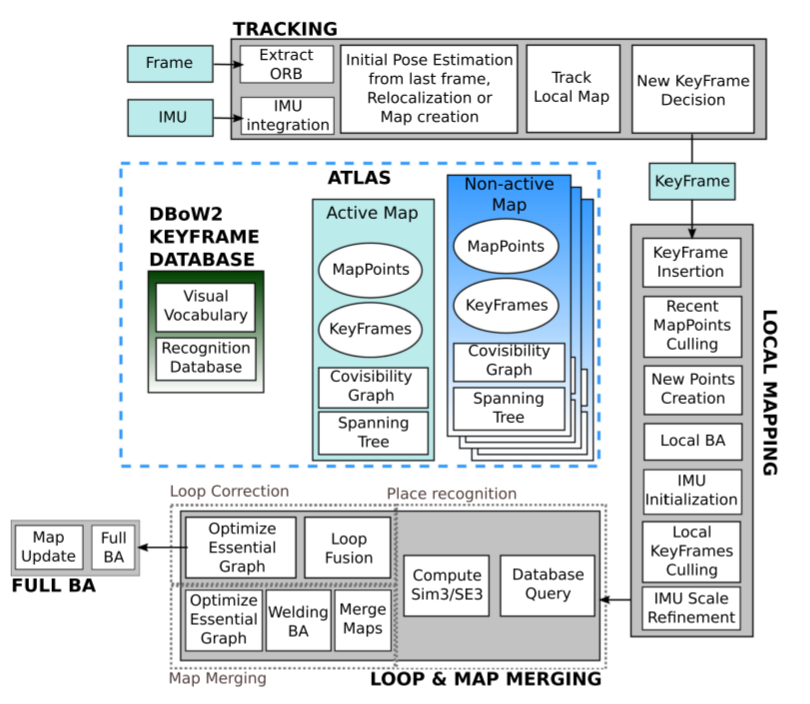
\includegraphics[scale=0.5]{orbslam.jpg}
\caption{The system overview of ORB-SLAM3 \cite{orbslam3}}
\label{fig_orbslam3}
\end{figure}


\subsection{Sensor Fusion and System Overview}
The visual–inertial SLAM system in ORB-SLAM3 performs graph-based combined adjustment by constructing a loss function consisting of the camera reprojection error and IMU preintegration error to optimize the system states and map points. Fig. \ref{fig_sensor_orbslam3} illustrates the sensor fusion of the visual–inertial SLAM system in ORB-SLAM3. Since the IMU and camera have different sampling rates, the IMU preintegration technique \cite{12} is used to avoid repeated IMU propagation. The preintegration is able to summarize several inertial measurements into a single relative motion constraint.

However, the problem is that the preintegration might enlarge the effect of IMU noise and bias when ORB-SLAM3 is used on NCLT dataset. Therefore, we would like to couple the wheel encoder to solve this problem. There are two ways to couple a wheel encoder in the system. The first way is to tightly couple the system with wheel encoder measurements. For example, as shown in Fig. \ref{fig_tightly}, we could first fuse the IMU and wheel encoder measurements to form the odometry information based on the method we discussed above, and then replace the IMU preintegration data with the odometry. 

\begin{figure}
\centering
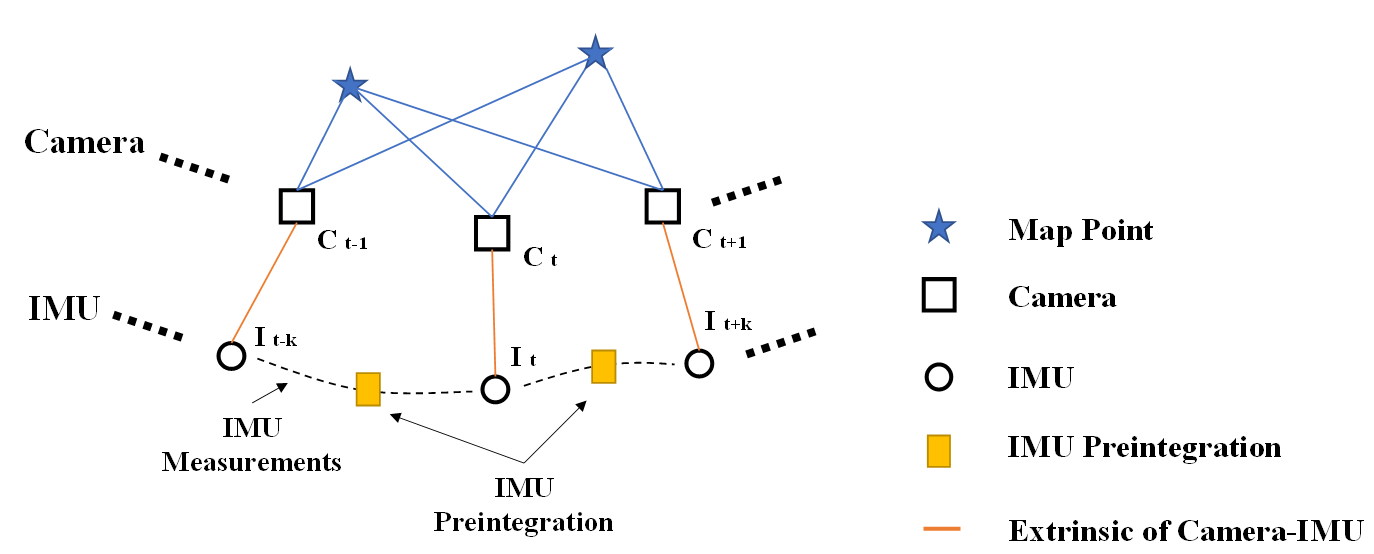
\includegraphics[scale=0.35]{Orb_sensor.PNG}
\caption{Illustration of the sensor fusion in the Visual–inertial SLAM system of ORB-SLAM3}
\label{fig_sensor_orbslam3}
\end{figure}

\begin{figure}
\centering
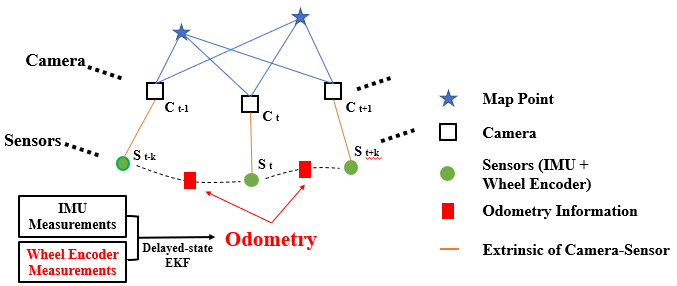
\includegraphics[scale=0.7]{tightly.PNG}
\caption{Tightly coupled with a wheel encoder}
\label{fig_tightly}
\end{figure}

The second way is to loosely couple wheel encoder measurements, which is our solution in this project. Fig. \ref{fig_system} shows the overall system of our work. The system first uses the sequence of pre-processed images and IMU measurements as inputs for the ORB-SLAM3. Then, the system takes the estimated trajectory
$X_1, X_2, ..., X_t$, where $X_k$ $(x_k,y_k,z_k,{roll}_k,{pitch}_k,{heading}_k)$ is generated by ORB-SLAM3 and the odometry information $O_1, O_2, ..., O_t$, where $O_k$ is $(O_{x_k},O_{y_k},O_{z_k},O_{{roll}_k},O_{{pitch}_k},O_{{heading}_k})$, to do the graph optimization and output the optimized trajectory. In this project, we used the poses estimated from ORB-SLAM3 to build the value instances in the factor graph. Then, we constructed the factors using odometry information. Finally, we conducted non-linear optimization based on the incremental smoothing technique (iSAM2) \cite{isam2} using the GTSAM library \cite{gtsam}.

\begin{figure*}
\centering
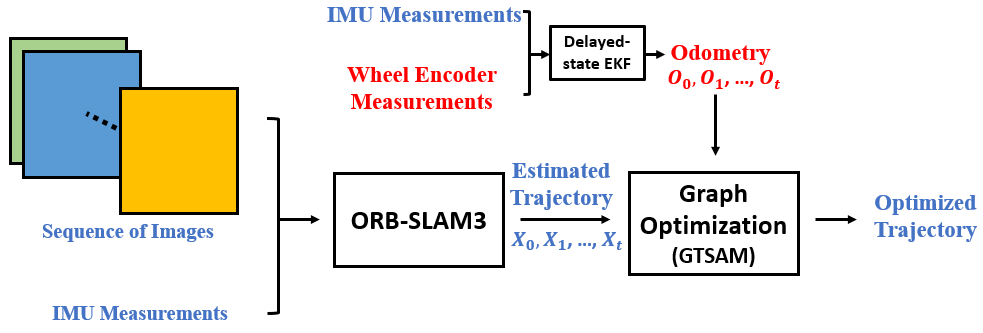
\includegraphics[scale=0.8]{System.PNG}
\caption{The system overview of our work}
\label{fig_system}
\end{figure*}

\section{EXPERIMENTS}

\subsection{Pre-processing of images in NCLT dataset} 
Images captured by the Ladybug3 camera are not ideal because of the imperfection from its pinhole camera nature. There is significant distortion in the pictures which severely downgrades the accuracy of the visual odometry estimated from the ORB features. Although ORB-SLAM3 natively supports undistortion configuration in 3 types of camera models, Ladybug3's distortion does not fall within any of these categories. Therefore, image pre-processing, as shown in Fig. \ref{fig_image_preprocess},  is required to improve the performance of the ORB-SLAM3 on the NCLT dataset. Fortunately, the NCLT dataset has provided the rectified map. This map relates each pixel in undistorted image $\mathbf{img}_{\textit{u}}(x,y)$ to a position on the original distorted image $\mathbf{img}_{\textit{d}}(x,y)$, and we can undistort the image beforehand using this map.
\begin{equation}
\mathbf{img}_{\textit{u}}(x,y)=\mathbf{img}_{\textit{d}}(map_x(x,y),\,map_y(x,y))
\end{equation}


However, undistortion also raises another problem: The output image has black margins around it, and the ORB feature extractor will generate false positives along the margins. Thus, these margins are cropped during the pre-processing. Moreover, the original orientation of the images is sideways, and the resolution is excessive. So the image should also be downsampled and rotated by 90 degrees. The pre-processing also influences the camera configuration of the ORB-SLAM3, which will be discussed in the following section.

\begin{figure}[ht]
\centering
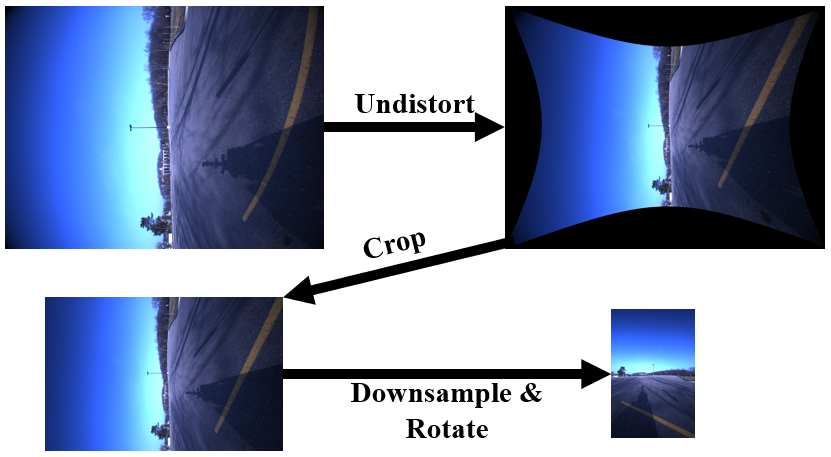
\includegraphics[height=3.6cm]{image_preprocess.png}
\caption{The workflow of image pre-processing}
\label{fig_image_preprocess}
\end{figure}


\subsection{Transformation Matrix}

\begin{figure}[ht]
\centering
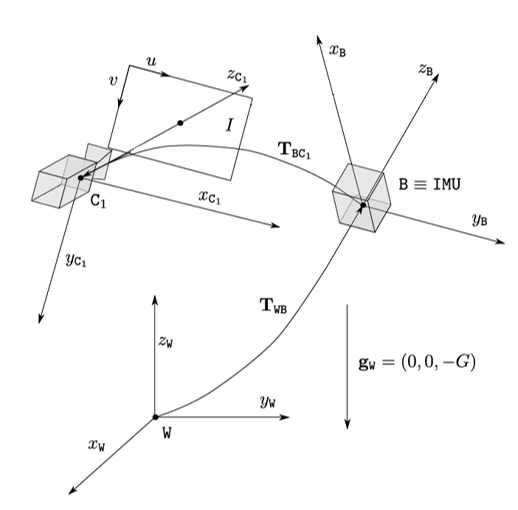
\includegraphics[height=4.5cm]{frame_orbslam.png}
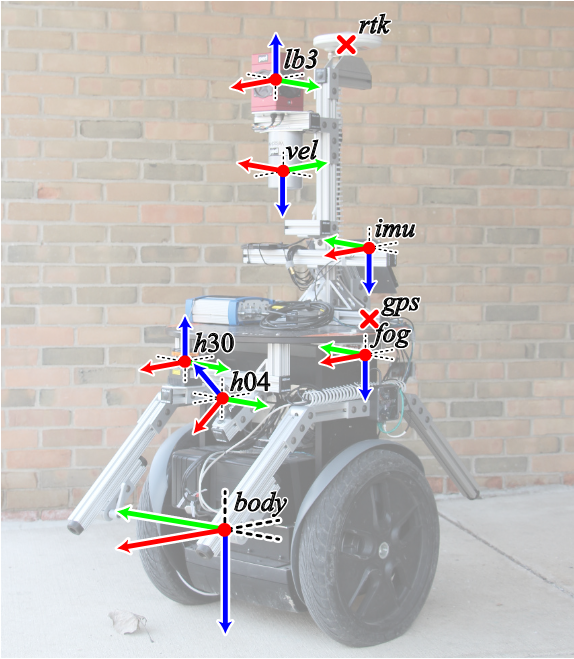
\includegraphics[height=4.5cm]{frame_nclt.png}
\caption{ORB-SLAM3's (left) and NCLT's (right) sensor frame definition \cite{orbslam3}\cite{NCLT}}
\label{fig_frame}
\end{figure}


For the monocular-inertial slam, ORB-SLAM3 needs the transformation matrix from the camera frame to the body frame, as shown in Fig. \ref{fig_frame}. However, the transformation between each frame defined by the NCLT dataset is presented in the 6 DOF format $\mathbf{x}_{i j}$. So, we should calculate the transformation matrix $\mathrm{T}_{ij}$ from 6 DOF by the following equation:

\begin{align}
\begin{split}
    \mathbf{x}_{i j}&=\left[ \mathbf{t}_{i j}^{\top}, \mathbf{\Theta}_{i j}^{\top}\right]^{\top}=\left[x_{i j}, y_{i j}, z_{i j}, \phi_{i j}, \theta_{i j}, \psi_{i j}\right]^{\top}\\
    \mathrm{R}_{ij} &=\operatorname{rotxyz}\left(\boldsymbol{\Theta}_{i j}\right) \\
    &=\operatorname{rotz}\left(\psi_{i j}\right)^{\top} \operatorname{roty}\left(\theta_{i j}\right)^{\top} \operatorname{rotx}\left(\phi_{i j}\right)^{\top} \\ \mathrm{T}_{ij}&=\left[\begin{array}{cc}
 \mathrm{R}_{ij} & \mathbf{t}_{i j} \\
\mathbf{0}^{\top} & 1
\end{array}\right]
\end{split}
\end{align}

The definitions of body frame are different in ORB-SLAM3 and NCLT. The body frame of ORB-SLAM3 is equivalent to the IMU frame while the origin of NCLT’s body frame is between two wheels. Moreover, an additional rotation matrix along the z-axis is required in consideration of the 90-degree rotation in the image pre-processing. The required transformation matrix is given by the following equation.

\begin{equation}
\mathrm{T}_{I C}=\mathrm{T}_{B I}^{-1} \mathrm{~T}_{B L} \mathrm{~T}_{L C} \operatorname{rotz}\left(-90^{\circ}\right)
\end{equation}

\subsection{ORB-SLAM3 Configuration}

For camera configuration, the image pre-processing should
be taken into account. The cropped black margin pixels are
reduced in the image shape and central point parameters.
Due to the downsampling, all the intrinsic parameters are
divided by two. Not all IMU noise parameters
are available in the manufacturer’s manual \cite{3DM-GX3-45}. Therefore, the random walks of the accelerometer and gyroscope are referred from Quinchia and Falco's research on the error model of 3DM-GX3-45 \cite{IMU_error}.

\begin{table}[ht]
\caption{The configuration of ORB-SLAM3}
\label{tab_orbslam_config}
\begin{tabular}{||l|l||}
\hline
Parameter                                & Value                                     \\ \hline
Focal   length (fx, fy):                 & (201.960408, 201.960408)                  \\ \hline
Central point (cx, cy):                  & (197.464760, 318.635272)                  \\ \hline
Distortion parameter (k1$\sim$3, p1, p2) & 0                                         \\ \hline
Camera width                             & 404                                       \\ \hline
Camera height                            & 624                                       \\ \hline
IMU accelerometer noise   density        & 7.84e-4 m/s\textasciicircum{}1.5          \\ \hline
IMU gyroscope noise density              & 5.235987756e-5 rad/s\textasciicircum{}0.5 \\ \hline
IMU Frequency                            & 50 Hz                                     \\ \hline
IMU accelerometer random walk            & 1.2e-4 m/s   \textasciicircum{}2.5        \\ \hline
IMU gyroscope random walk                & 7.6e-4 rad/s   \textasciicircum{}1.5      \\ \hline
\end{tabular}
\end{table}


\subsection{Graph-Optimization-Based Sensor Fusion} 

In this project, we loosely couple the wheel encoder information into the system based on the method mentioned in the methodology section. The sensor fusion is off-line and is used to optimize the ORB-SLAM3 estimated poses. The first 726 estimated poses are used to build the value instances in the factor graph, and the corresponding odometry information is used to construct the factors. The first pose generated by ORB-SLAM3 is at the origin $X_0$ ($x_0,y_0,z_0,{roll}_0,{pitch}_0,{heading}_0$ = 0,0,0,0,0,0). However, the ground-truth pose of the corresponding timestamp is not at the origin. Therefore, we first use the corresponding ground-truth pose $ X_{gt0} (x_{gt0},y_{gt0},z_{gt0},{roll}_{gt0},{pitch}_{gt0},{heading}_{gt0})$ and $X_0$ to generate the transformation matrix $T$. Then, we transform the estimated poses to make the estimated poses and the ground-truth poses in the same reference coordinate by following the equation 
\begin{equation}
\mathrm{X_t'}=\mathrm{T}^{-1} \mathrm{X_t}
\end{equation}
Afterward, we use a nonlinear factor graph as our graph and use the ISAM2 solver to optimize the trajectory incrementally.


\section{RESULTS AND DISSCUSSIONS}

\subsection{Challenges of Using ORB-SLAM3 on NCLT Dataset}
The NCLT dataset has presented various challenges to the visual slam algorithm like low frame rate, high speed, sparse reference, outdoor environment, etc., which leads to the failure of the original ORB-SLAM3 in the localization.

The first problem is losing track of the local map. Due to the high speed of the robot, low image frequency, and the sparse scenes, likely, the algorithm cannot find any matched feature points between 
two adjacent frames. The outdoor environment is also a big challenge. Sometimes, the reference objects are too far away and do not move much between frames, making it hard to calculate the visual odometry correctly. We have also observed several cases where the ORB extractor captures some features on the shadow of the robot, as shown in Fig. \ref{fig_feature_on_shadow}, which may cause a false estimation of the camera poses. From our experiment, these problems make it impossible for OBR-SLAM3 in monocular-only mode to output any reasonable estimation of the camera trajectory. 

\begin{figure}[h]
\centering
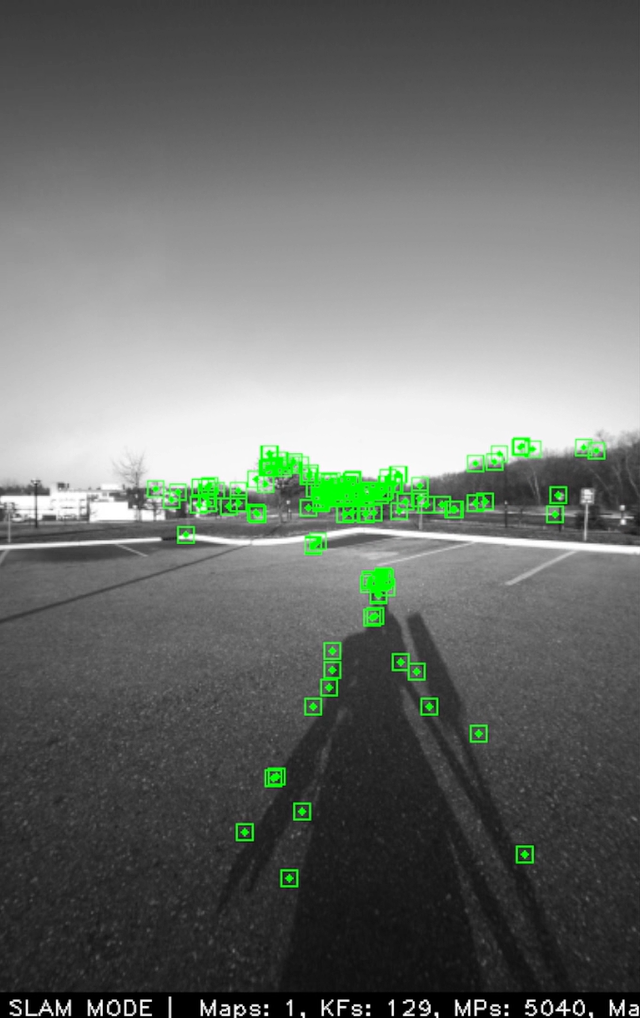
\includegraphics[height=6cm]{feature_on_shadow.png}
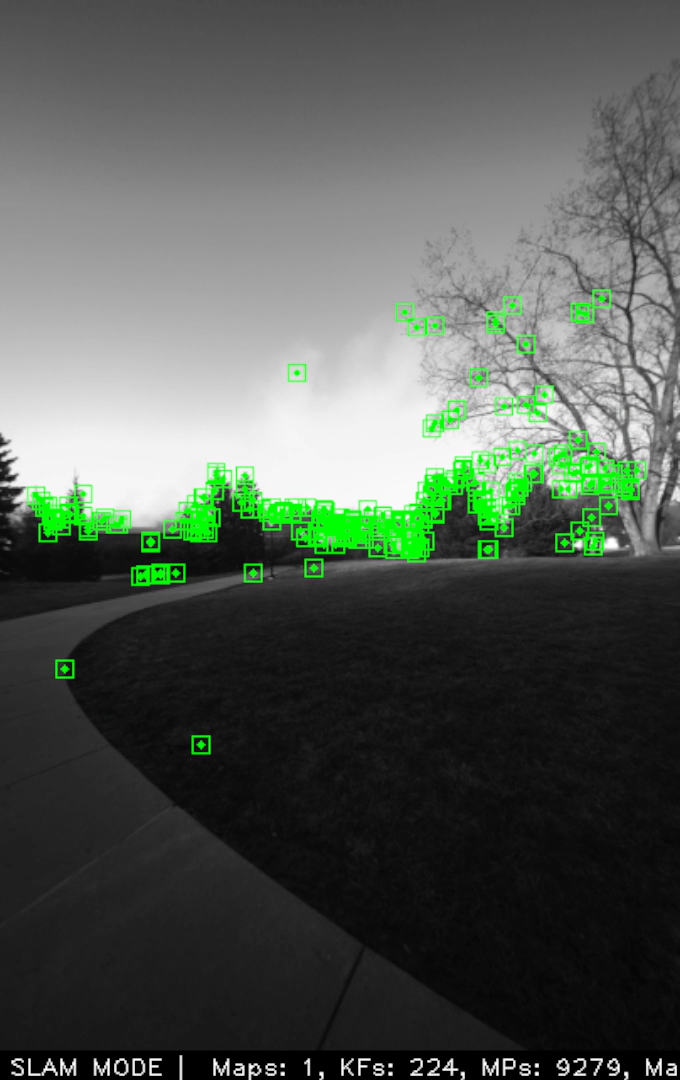
\includegraphics[height=6cm]{foliage.png}
\caption{These features on the shadow (left) and foliage (right) cause ORB-SLAM3 to generate wrong visual odometries}
\label{fig_feature_on_shadow}
\end{figure}

However, even in the monocular-inertial mode that ORB-SLAM3 natively supports the accuracy of localization still suffers from the noise and the bias of the IMU measurement, causing the incorrect scale of the estimated trajectory and the erroneously estimated angles during turning around. An extreme case of failure happens when the robot stops with only foliage far away inside the view. Static pose causes the noise and bias to accumulate while the foliage in the view generates noisy features and erroneous visual odometry, which leads to a drastic drift of the estimated trajectory, as shown in Fig. \ref{fig_feature_on_shadow}.


Fortunately, our experiment has also proved that these issues can be solved by introducing the wheel encoder into the sensor fusion.


\subsection{Results}
To evaluate our results, we plot two trajectories: one is generated by ORB-SLAM3, and the other is generated by our method, which applies sensor fusion using graph optimization to the previous trajectory. We also provide the Root Mean Square Error (RMSE) in both x and y dimensions and the Average Displacement Error (ADE) to evaluate the accuracy of the trajectories. The Average Displacement Error (ADE) is the average value of euclidean distances between all the estimated poses and the ground truth poses.
By comparing to the ground truth, it is evident that the robustness and estimation accuracy of our method is much better. As shown in Fig. \ref{fig_result}, the "ORB-SLAM3 Trajectory" converges initially but deviates soon and hardly converges to ground truth afterward. This is because there is a sharp turn, which disables the continuous tracking of reference points. Also, there is a spike in the second turn, which results from the extreme case when the robot stops in front of some foliage. As a result, as observed in the "ORB-SLAM3 Trajectory", the ORB-SLAM3 loses track of location information on the NCLT dataset. Besides, as shown in Table \ref{table_rmse}, our method solves the lost tracking problem of the ORB-SLAM3 and merely has around a one-meter displacement error with the ground truth.
\begin{figure}[ht]
\centering
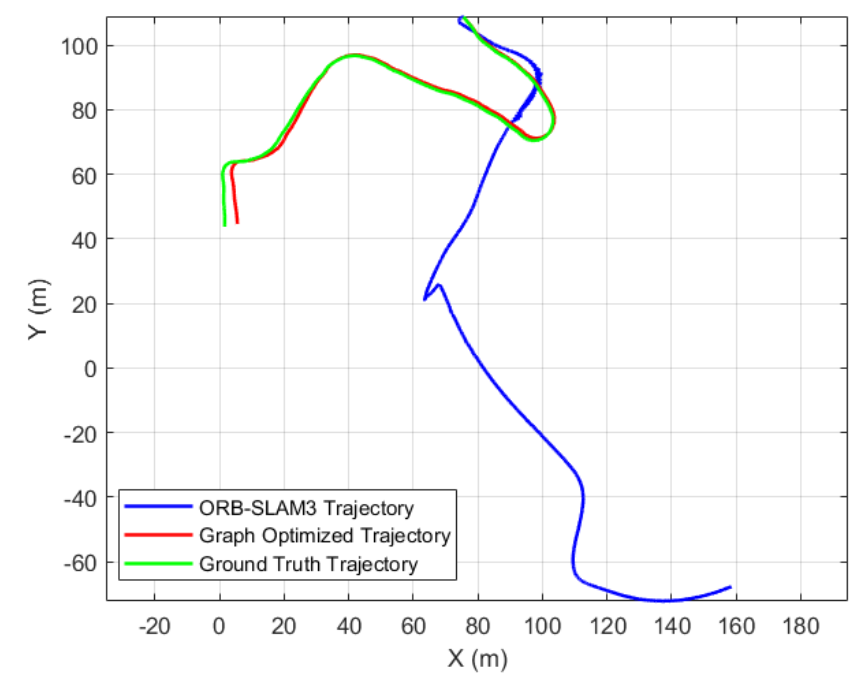
\includegraphics[scale=0.36]{result.png}
\caption{Result trajectories and ground truth}
\label{fig_result}
\end{figure}
For "Graph optimized trajectory", it can be observed that the robot can pickup its location when there is sharp turn. This trajectory converges to the ground truth and able to reflect an authentic position information of the robot.

More information can be found in our project presenation video: \href{https://youtu.be/nWXb3qt6gEo}{https://youtu.be/nWXb3qt6gEo}.

\begin{table}[ht]
\caption{Evaluation metrics of each methods}
\label{table_rmse}
\begin{center}
\begin{tabular}{||c|c|c||}
\hline
 Error Type & ORB-SLAM3 & Our Method\\
\hline
RMSE in x & 55.725 m & 1.399 m\\
\hline
RMSE in y &67.204 m & 0.546 m\\
\hline
ADE & 61.732 m  & 1.062 m \\
\hline
\end{tabular}
\end{center}
\end{table}


\section{CONCLUSIONS}

In this project, we first run ORB-SLAM3 on the NCLT dataset. However, even though we properly pre-process data in the NCLT dataset, the ORB-SLAM3 fails in the challenging environment of the NCLT dataset. The estimated trajectory drastically diverge from the ground truth. Therefore, we propose an improvement to the ORB-SLAM3 by fusing the estimation trajectory with the odometry calculated from the IMU and wheel encoder on the robot. The IMU and wheel encoder provide real-time information on the robot's acceleration and linear and angular velocity, which improve the robustness and accuracy of the estimation. As a result, by comparing two estimated trajectories with the ground truth, we observe that the trajectory generated by our method has higher accuracy than the original trajectory of ORB-SLAM3. Furthermore, it can be observed that the sensor fusion is capable of generating trajectories with higher accuracy. For our future work, we can implement tightly coupled sensor fusion and also introduce extra sensors in the algorithm to improve its performance.


\addtolength{\textheight}{-12cm}   % This command serves to balance the column lengths
                                  % on the last page of the document manually. It shortens
                                  % the textheight of the last page by a suitable amount.
                                  % This command does not take effect until the next page
                                  % so it should come on the page before the last. Make
                                  % sure that you do not shorten the textheight too much.

%%%%%%%%%%%%%%%%%%%%%%%%%%%%%%%%%%%%%%%%%%%%%%%%%%%%%%%%%%%%%%%%%%%%%%%%%%%%%%%%



%%%%%%%%%%%%%%%%%%%%%%%%%%%%%%%%%%%%%%%%%%%%%%%%%%%%%%%%%%%%%%%%%%%%%%%%%%%%%%%%



%%%%%%%%%%%%%%%%%%%%%%%%%%%%%%%%%%%%%%%%%%%%%%%%%%%%%%%%%%%%%%%%%%%%%%%%%%%%%%%%

\newpage

\begin{thebibliography}{99}
\bibitem{intro} T. Taketomi, H. Uchiyama and S. Ikeda, "Visual SLAM algorithms: a survey from 2010 to 2016," \textit{IPSJ Transactions on Computer Vision and Applications}, 9(1), 2017.
\bibitem{1} D. Scaramuzza and F. Fraundorfer, “Visual Odometry [Tutorial],” \textit{IEEE Robot. Autom. Mag.}, vol. 18, no. 4, pp. 80–92, 2011.
\bibitem{2} F. Fraundorfer and D. Scaramuzza, “Visual odometry: Part II: Matching, robustness, optimization, and applications,” \textit{IEEE Robot. Autom. Mag.}, vol. 19, no. 2, pp. 78–90, 2012.
\bibitem{3} F. Jiang, J. Chen, and S. Ji, “Panoramic visual-inertial SLAM tightly coupled with a wheel encoder,” \textit{ISPRS J. Photogramm. Remote Sens.}, vol. 182, pp. 96–111, 2021.
\bibitem{orbslam3}	C. Campos, R. Elvira, J. J. G. Rodriguez, J. M. M. Montiel, and J. D. Tardos, “ORB-SLAM3: An accurate open-source library for visual, visual–inertial, and multimap SLAM,” \textit{IEEE Trans. Robot.}, vol. 37, no. 6, pp. 1874–1890, 2021.
\bibitem{Mouragon} E. Mouragnon, M. Lhuillier, M. Dhome, F. Dekeyser, and P. Sayd, “Real time localization and 3D reconstruction,” in \textit{2006 IEEE Computer Society Conference on Computer Vision and Pattern Recognition (CVPR’06)}, 2006.
\bibitem{Klein} G. Klein and D. Murray, “Parallel tracking and mapping for small AR workspaces,” in \textit{2007 6th IEEE and ACM International Symposium on Mixed and Augmented Reality}, 2007.
\bibitem{7} R. Mur-Artal, J. M. M. Montiel, and J. D. Tardos, “ORB-SLAM: A versatile and accurate monocular SLAM system,” \textit{IEEE Trans. Robot.}, vol. 31, no. 5, pp. 1147–1163, 2015.
\bibitem{8} T. Qin, P. Li, and S. Shen, “VINS-mono: A robust and versatile monocular visual-inertial state estimator,” \textit{IEEE Trans. Robot.}, vol. 34, no. 4, pp. 1004–1020, 2018.
\textit{Int. J. Rob. Res.}, vol. 33, no. 2, pp. 207–214, 2014.
\bibitem{12} C. Forster, L. Carlone, F. Dellaert, and D. Scaramuzza, “IMU Preintegration on Manifold for Efficient Visual-Inertial Maximum-a-Posteriori Estimation,” in  \textit{Robotics: Science and Systems XI}, 2015.
\bibitem{euroc} M. Burri et al., “The EuRoC micro aerial vehicle datasets,” \textit{Int. J. Rob. Res.}, vol. 35, no. 10, pp. 1157–1163, 2016.
\bibitem{tumvi} [6]	D. Schubert, T. Goll, N. Demmel, V. Usenko, J. Stuckler, and D. Cremers, “The TUM VI benchmark for evaluating visual-inertial odometry,” in \textit{2018 IEEE/RSJ International Conference on Intelligent Robots and Systems (IROS)}, 2018.
\bibitem{NCLT}	N. Carlevaris-Bianco, A. K. Ushani, and R. M. Eustice, “University of Michigan North Campus long-term vision and lidar dataset,” \textit{Int. J. Rob. Res.}, vol. 35, no. 9, pp. 1023–1035, 2016.
\bibitem{11} J.-L. Blanco-Claraco, F.-Á. Moreno-Dueñas, and J. González-Jiménez, “The Málaga urban dataset: High-rate stereo and LiDAR in a realistic urban scenario,” \textit{Int. J. Rob. Res.}, vol. 33, no. 2, pp. 207–214, 2014.
\bibitem{14} M. Fallon, H. Johannsson, M. Kaess, and J. J. Leonard, “The MIT Stata Center dataset,” \textit{Int. J. Rob. Res.}, vol. 32, no. 14, pp. 1695–1699, 2013.
\bibitem{delayed-state framework} R. M. Eustice, H. Singh, and J. J. Leonard, “Exactly sparse delayed-state filters for view-based SLAM,” \textit{IEEE Trans. Robot.}, vol. 22, no. 6, pp. 1100–1114, 2006.
\bibitem{tail-to-tail} R. Smith, M. Self, and P. Cheeseman, “Estimating uncertain spatial relationships in robotics,” in \textit{Proceedings. 1987 IEEE International Conference on Robotics and Automation}, 2005.
\bibitem{orbslam2} R. Mur-Artal and J. D. Tardos, “ORB-SLAM2: An open-source SLAM system for monocular, stereo, and RGB-D cameras,” \textit{IEEE Trans. Robot.}, vol. 33, no. 5, pp. 1255–1262, 2017.
\bibitem{orbslamVI} R. Mur-Artal and J. D. Tardos, “Visual-inertial monocular SLAM with map reuse,” \textit{IEEE Robot. Autom. Lett.}, vol. 2, no. 2, pp. 796–803, 2017.
\bibitem{isam2} M. Kaess, H. Johannsson, R. Roberts, V. Ila, J. J. Leonard, and F. Dellaert, “iSAM2: Incremental smoothing and mapping using the Bayes tree,” \textit{Int. J. Rob. Res.}, vol. 31, no. 2, pp. 216–235, 2012.
\bibitem{gtsam} F. Gtsamdellaert, \textit{Factor graphs and GTSAM: A hands-on introduction}. 2012.
\bibitem{3DM-GX3-45} Microstrain, Inc, “3DM-GX3-45 Theory of Operation,” 2012.
\bibitem{IMU_error}	A. G. Quinchia, G. Falco, E. Falletti, F. Dovis, and C. Ferrer, “A comparison between different error modeling of MEMS applied to GPS/INS integrated systems,” \textit{Sensors (Basel)}, vol. 13, no. 8, pp. 9549–9588, 2013.







\end{thebibliography}




\end{document}
